\title{Throughput-Optimal Scheduling in Wireless Systems with Quality of Experience Constraints}
\author{Kishan P. B. and Basty Ajay Shenoy}
\date{ }

\documentclass[10pt,a4paper]{article}
%% \usepackage{hyperref}[2010/09/11]
% \usepackage{amssymb}
%\usepackage{amsmath}
%\usepackage{wasysym}
%\usepackage{amsthm}
%\usepackage{enumerate}
% \usepackage{graphicx,psfrag} % for jpg, jpeg, bitmapped graphics files
% \usepackage{times}
%%\paperheight = 950pt 
% \textheight = 650pt
% \voffset = -35pt
% \hoffset = 0pt
%\marginparwidth = 0pt
%%\textwidth = 390pt
%\marginparsep = 0pt
%% \headsep = 15pt
%
%
%\theoremstyle{plain}
%\newtheorem{thm}{{Theorem}}
%\newtheorem{lem}{{Lemma}}
%\newtheorem{prop}{Proposition}
%\newtheorem{cor}{Corollary}
%
%
%
%
%
%
%\theoremstyle{definition}
%\newtheorem{defn}{Definition}
%\newtheorem{conj}{Conjecture}[section]

\usepackage{%
	amsfonts,%
	amsmath,%	
	etex,%
	amssymb,%
	amsthm,%
	babel,%
	bbm,%
	%biblatex,%
	caption,%
	centernot,%
	color,%
	enumerate,%
	epsfig,%
	epstopdf,%
	geometry,%
	graphicx,%
	hyperref,%
	latexsym,%
	mathtools,%
	multicol,%
	pgf,%
	pgfplots,%
	pgfplotstable,%
	pgfpages,%
	proof,%
	psfrag,%
	subfigure,%	
	tikz,%
	ulem,%
	url%
}	

\usepackage[mathscr]{eucal}
\usepgflibrary{shapes}
\usetikzlibrary{%
  arrows,%
	backgrounds,%
	chains,%
	decorations.pathmorphing,% /pgf/decoration/random steps | erste Graphik
	decorations.text,%
	matrix,%
  	positioning,% wg. " of "
  	fit,%
	patterns,%
  	petri,%
	plotmarks,%
  	scopes,%
	shadows,%
  	shapes.misc,% wg. rounded rectangle
  	shapes.arrows,%
	shapes.callouts,%
  	shapes%
}

\theoremstyle{plain}
\newtheorem{thm}{Theorem}[section]
\newtheorem{lem}[thm]{Lemma}
\newtheorem{prop}[thm]{Proposition}
\newtheorem{cor}[thm]{Corollary}

\theoremstyle{definition}
\newtheorem{defn}[thm]{Definition}
\newtheorem{conj}[thm]{Conjecture}
\newtheorem{exmp}[thm]{Example}
\newtheorem{assum}[thm]{Assumptions}
\newtheorem{axiom}[thm]{Axiom}

\theoremstyle{remark}
\newtheorem{rem}{Remark}
\newtheorem{note}{Note}

\newcommand{\norm}[1]{\left\lVert#1\right\rVert}
\newcommand{\indep}{\!\perp\!\!\!\perp}
\DeclarePairedDelimiter\abs{\lvert}{\rvert}%
%\DeclarePairedDelimiter\norm{\lVert}{\rVert}%
\newcommand{\tr}{\operatorname{tr}}
\newcommand{\R}{\mathbb{R}}
\newcommand{\Q}{\mathbb{Q}}
\newcommand{\N}{\mathbb{N}}
\newcommand{\E}{\mathbb{E}}
\newcommand{\Z}{\mathbb{Z}}
\newcommand{\B}{\mathscr{B}}
\newcommand{\C}{\mathcal{C}}
\newcommand{\T}{\mathscr{T}}
\newcommand{\F}{\mathcal{F}}
\newcommand{\G}{\mathcal{G}}
%\newcommand{\ba}{\begin{align*}}
%\newcommand{\ea}{\end{align*}}

\makeatletter
\def\th@plain{%
  \thm@notefont{}% same as heading font
  \itshape % body font
}
\def\th@definition{%
  \thm@notefont{}% same as heading font
  \normalfont % body font
}
\makeatother
\date{}

\begin{document}
\maketitle
\thispagestyle{empty}



\begin{abstract}
We address the problem of service allocation to two types of users of differing demands of service. Type 1 user is time conscious and Type 2 user is quality conscious. The service allocation takes into account these demands to ensure optimal quality of service, the optimality being dependent on the frustration levels of the individual users. We model the frustration of the Type 1 user in two ways. For the scenario where the Type 1 user leaves after $T$ consecutive seconds of not being served, we consider a priority max-weight allocation to ensure he does not leave. We then consider a scenario where he does not leave, but every set of consecutive non-service durations adds to frustration. We present optimum allocation taking into account stability conditions.
\end{abstract}



\section{Introduction}
We consider a network consisting of one base station and $2$ users requesting (video) data from the base station. Person A is time-sensitive, that is, he is disturbed by the buffering time of the video, and quality insensitive, that is, he is fine with lower resolution video. Person B is quality sensitive but time-insensitive. The adaptive allocation of the rate and the queue backlog at the base station is modeled as follows. Let $\{Q_i(t)\}, i \in \{1,2 \}$ be the packets in the buffers at the base station at time $t$, $\{a_i(t)\} , i \in \{1,2\}$ be the arrival process at the buffers, and $\{b_i(t)\}, i \in \{1,2\}$ be the allocation/service process.
The queues evolve as per the following:
\begin{align}
\label{eqn:QueueEvolution}
Q_i(t+1) = \max(Q_i(t)-b_i(t),0) + a_i(t),
\end{align}
which can equivalently be written as \eq{Q_i(t+1) = Q_i(t)-\tilde{b}_i(t) + a_i(t),} where $\tilde{b}_i(t) = \min(b_i(t),Q_i(t)).$
We denote by $\mu_i$ the rate of $b_i$ and by $\lambda_i$ the rate of the arrival process $a_i, i \in\{1,2\}.$ In this work, we consider the following stability requirements. %The following assumptions are made in the sequel: 

%
%
%\noindent $\lambda_i = E[a_i ]$, $\mu_i = E[b_i]$, for $i = 1,2.$    \\
%$\lambda_1 <1$, $\lambda_2<1$ and $\lambda_1 + \lambda_2<1$,  \\
%$\lambda_i < \mu_i$, for $i = 1,2.$
%



%\begin{defn}[Rate Stability]
A discrete-time process $Q(t)$ is {\it rate stable} if \eq{\lim_{t\to\infty} \frac{Q(t)}{t} = 0,}
%\end{defn}
and 
%\begin{defn}[Strongly Stable]
%A discrete-time process $Q(t)$ is 
{\it strongly stable} if \eq{\limsup_{t \to \infty} \frac{1}{t} \sum_{\tau=0}^t \E [|Q(\tau)|] <\infty.}
%\end{defn}

A necessary and sufficient condition for rate stability is the following \cite{neely2010stochastic}.
\begin{thm}
\label{thm:RateStability}
If $Q_i(t)$ evolves according to \eqref{eqn:QueueEvolution}, then it is rate stable if and only if $\lambda_i \leq \mu_i.$
\end{thm}
%In view of Theorem \ref{thm:RateStability}, we make the following assumptions in the sequel: $\lambda_i<1, \lambda_i<\mu_i, i = 1$ and $2$, $\lambda_1+\lambda_2<1.$

A sufficient condition for strong stability is the following Lyapunov criterion \cite{kumar2008wireless}.

\begin{thm}
\label{thm:LyapunovStability}
Let $L:\mathbb{Z}_+\to \mathbb{R}_+$ be an increasing function. If there exists  $\epsilon>0$ and $0<B<\infty$ such that \eq{\E[L(Q(t+1)) -L(Q(t))|Q(t)]\leq B-\epsilon Q(t),} then $Q(t)$ is strongly stable.
\end{thm}


\subsection{Problem Statement}
We address two problems in this work. The first is when the buffers are of finite length and the arrival processes $\{a_i\}$ have rates $\lambda_i, i\in\{1,2\}.$ Within this context, we assume that Person A leaves the system if he is not served for $T$ seconds, and the system incurs a loss, and the task is to minimise a corresponding cost function subject to rate stability.

In the second problem, we consider an infinite backlog queue and model the frustration of Person A to increase with the number of consecutive intervals he is not served. The task is to minimise the time average cost.


\subsection{Organization}
In Section \ref{sec:FiniteQueues}, we analyse finite-length queues with arrival rates $\lambda_i, i \in\{1,2\}$, where Person A leaves the system if he is not served for $T$ consecutive seconds. This is modeled as a loss to the system, and a priority max-weight allocation policy is developed, whose stability is established employing an appropriate Lyapunov function and corresponding simulation results pertaining to two types of arrival processes are presented. In Section \ref{sec:BacklogQueues}, we consider infinite backlog queues modelling the frustration of Person A via an appropriate convex increasing loss function to enhance an interleaved service. The renewal reward theorem converts the stochastic optimization problem to a deterministic one pertaining to the respective rates.





\begin{figure}[b]
\centering
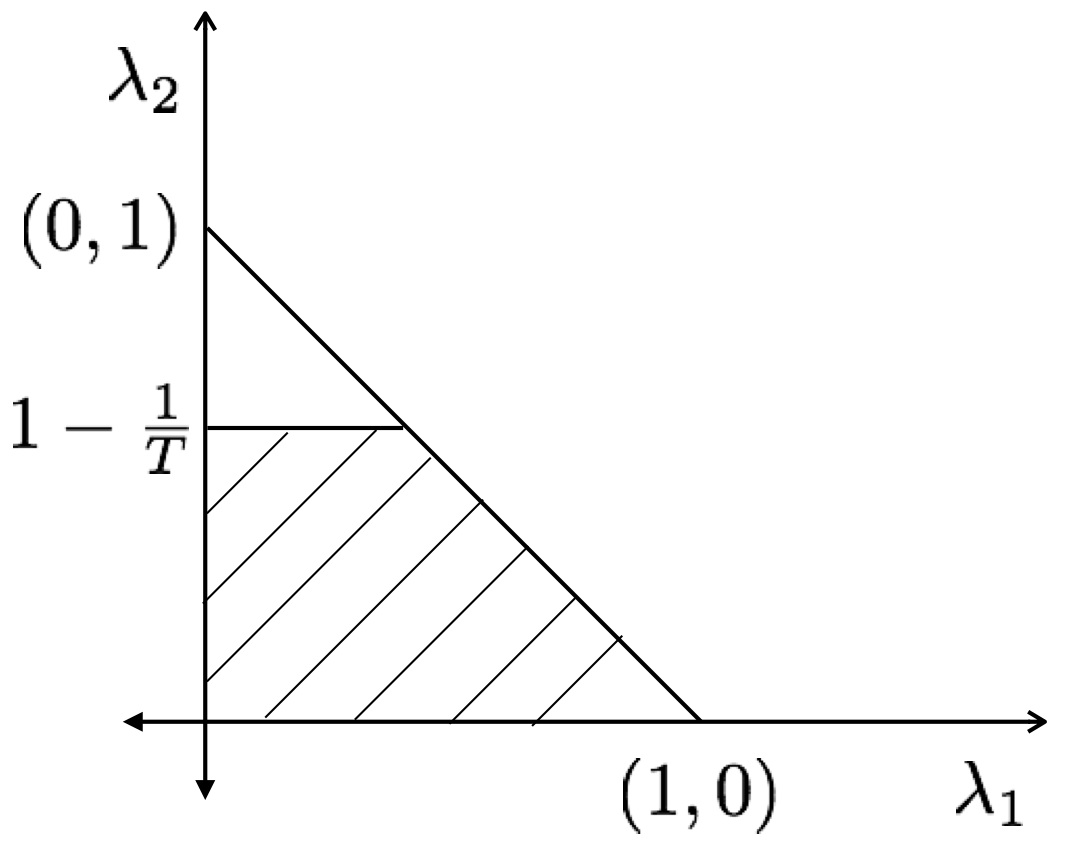
\includegraphics[width = 2.5in]{Figures/StabilityRange}
\caption{Stability Range}
\label{fig:StabilityRange}
\end{figure}

\section{Finite Queues }
\label{sec:FiniteQueues}
In this setup, Person A leaves if he is not served for $T$ consecutive seconds and hence a necessary condition for the allocation algorithm is $\mu_1\geq \frac{1}{T}.$ Now since $b_1 + b_2 = 1$, it follows that $\mu_2\leq 1-\frac{1}{T}$. In view of Theorem \ref{thm:RateStability}, we need $\lambda_2 < \mu_2\leq1-\frac{1}{T}$ for rate stability.
The stability region in terms of arrival rates thus becomes 
\begin{align*}
\left\{(\lambda_1,\lambda_2): \lambda_1+ \lambda_2 <1, \lambda_1<1, \lambda_2 < 1-\frac{1}{T}\right\},
\end{align*}
as indicated in Figure \ref{fig:StabilityRange}.



%
%\subsection*{Area  maximization:}
%
%\subsection*{Where max-weight fails:}
%



\subsection{A Cost Based Approach}
We can consider a cost minimisation problem where we incur a cost for losing Person A and a cost for delaying service to Person B. Towards this end, we define the stopping time 
\begin{align*}
Y = \text{min }\big\{t: \{b(t-j)\}_{j=0}^{T-1} = (0,\cdots,0) \big\},
\end{align*}
that is, $Y$ is the time instant when Person A leaves. Accordingly, we can consider the cost 
\begin{align*}
\gamma_1(t) = f(Y)\mathbf{1}_{\{t\geq Y\}},
\end{align*} 
where $f$ is an appropriate non-decreasing function. 


The cost pertaining to Person B is 
\begin{align}
\label{eqn:CostB}
\gamma_2(t) = \{ \text{number of $0$'s in } \{b_2(\tau)\}_{\tau=0}^t\}.
 \end{align}
An appropriate weighing of these two costs will provide us with the total cost: $C(t) = \alpha_1 \gamma_1(t) + \alpha_2 \gamma_2(t)$, and the following minimisation problem can be addressed

\begin{equation*}
\begin{array}{lc}
\text{Minimize } & C(t) \\
\text{Subject to } & \text{Stability.}
\end{array}
\end{equation*}


A special case of this minimisation problem is to ensure that Person A never leaves. This can be done by choosing $\alpha_1 = \infty$, in which case we obtain the following equivalent minimisation problem
\begin{equation*}
\begin{array}{lc}
\text{Minimize } & \gamma_2(t) \\
\text{Subject to } & \text{Stability} \\
~& \gamma_1(t) = 0.
\end{array}
\end{equation*}
This can be solved by employing a {\it priority max-weight} scheduling policy as follows. For every $t=nT+1$ for some integer $n$, let $b_1(t) = 1$, and for all other $t$, employ the max-weight allocation. 




\begin{figure}[t]
$\begin{array}{cc}
\centering
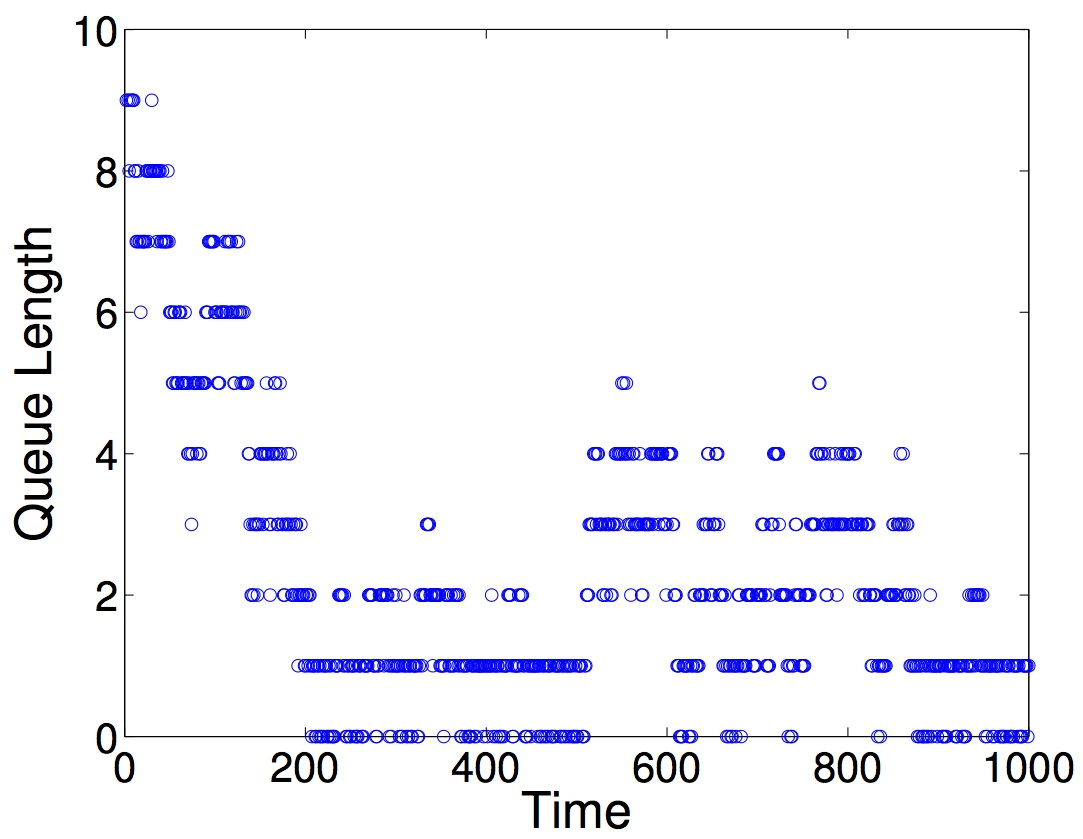
\includegraphics[width = 2.75in]{Figures/Bernoulli_1.jpg} &
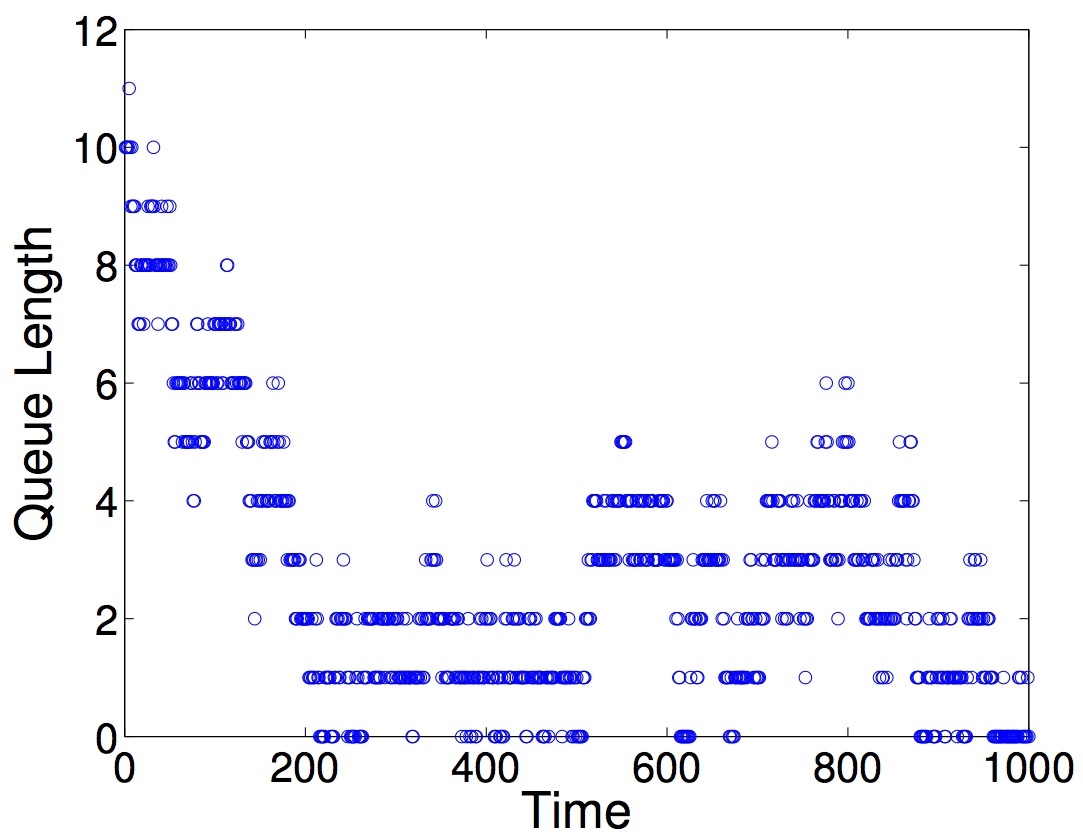
\includegraphics[width = 2.75in]{Figures/Bernoulli_2.jpg} \\
(a) & (b)
\end{array}$
\caption{Queue lengths as a function of time for (a) $Q_1$ and (b) $Q_2$ for the priority max weight allocation with Bernoulli arrival process with $p_1 = 0.6$ and $p_2 = 0.3$.}
\label{fig:Bernoulli}
\end{figure}




\subsection{Stability and the Lyapunov Drift}
To see that the priority max-weight allocation is stable, we consider the Lyapunov functions $L_i(Q_i(t)) = Q_i^2(t), i = 1$ and $2$. Generalizing Theorem \ref{thm:LyapunovStability} to $T$-slot drift, we have that $Q_i(t)$ is strongly stable if there exists $T$, $0<B<\infty$, and $\epsilon>0$ such that 
\begin{align*}
\E(L(Q_i(t_0+T)) - L(Q_i(t_0))| Q_i(t_0)) \leq B - \epsilon Q_i(t_0)
\end{align*}
We obtain an upper bound on $Q_i(t_0+T)$ as follows. Assume that in slots $t_0,\cdots, t_0+T-1$, we serve only those packets that were in the system till $t_0.$ Since in each slot, at most $1$ packet can be served, we have that $Q_i(t_0)$ can decrement by at most $T$. In the slots $t_0+1, \cdots, t_0+T$, at most $T$ packets can have arrived, we have 
\begin{align} Q_i(t_0+T) \leq \max \left( Q_i(t_0) - \sum_{t_0}^{t_0+T-1} b_i(t) ,0 \right) + \sum_{t=t_0+1}^{t_0+T} a_i(t)  \label{eqn:Qinequality}
\end{align}
To proceed, we need the following result \cite{kumar2008wireless}.
\begin{lem}
\label{lem:Maxinequality}
If $W\leq \max(X-Y,0)+Z$, then $W^2\leq X^2+Y^2+Z^2-2X(Y-Z).$
\end{lem}
\noindent From \eqref{eqn:Qinequality} and Lemma \ref{lem:Maxinequality}, we have 
\begin{align*}
Q_i^2(t_0+T) \leq Q_i^2(t_0)+2T^2 - 2T Q_i(t_0)\left(\frac{1}{T}\sum_{t=t_0}^{t_0+T-1}b_i(t) -\frac{1}{T}\sum_{t=t_0+1}^{t_0+T} a_i(t) \right).
\end{align*}
Taking expectations conditioned on $Q_i(t_0)$, we get
\begin{align*}
&\E(Q_i^2(t_0+T)-Q_i^2(t_0)|Q_i(t_0) )\\
&~~~~\leq 2T^2 - 2T Q_i(t_0) \left(\E  \left(\frac{1}{T}\sum_{t=t_0}^{t_0+T-1}b_i(t) |Q_i(t_0)\right) -\E\left(\frac{1}{T}\sum_{t=t_0+1}^{t_0+T} a_i(t)|Q_i(t_0)\right) \right)\\
&~~~~\leq 2T^2 - 2TQ_i(t_0) \left( \mu_i-\lambda_i-2\epsilon_1\right) \\
&~~~~ = B - (\epsilon^{i}_2-2\epsilon_1) 2TQ_i(t_0)\\
&~~~~ = B - \epsilon Q_i(t_0),
\end{align*}
where $\epsilon^{i}_2 :=\mu_i -\lambda_i $, $B := 2T^2$, $\epsilon := (\epsilon^{i}_2-2\epsilon_1)2T$, and $\epsilon_1$ is such that \eq{  \E\left(\frac{1}{T} \sum_{t=t_0}^{t_0+T-1}a_i(t)|Q_i(t_0)\right) &\leq \lambda_i+\epsilon_1 \\  \E\left(\frac{1}{T}\sum_{t=t_0}^{t_0+T-1}b_i(t)|Q_i(t_0)\right) &\geq \mu_i-\epsilon_1,}
which shows that both the queues are stable.



\subsection{Simulation Results}

%[Bernoulli, deterministic]

We simulate the priority max-weight allocation policy for the cases where the arrivals are Bernoulli and deterministic.

For the Bernoulli arrivals, we let $a_i(t) \sim \mathrm{Bernoulli}(p_i), i = 1$ and $2$. When $p_1+p_2<1$, the queues are stable. Starting with queue lengths of $10$ each, a typical realisation of the priority max weight is shown in Figure \ref{fig:Bernoulli} for $p_1 = 0.6 $ and $p_2 = 0.3$. When $p_1+p_2>1$, the queues are not stable. In Figure \ref{fig:BernoulliUnstable}, we consider $p_1 = 0.6$ and $p_2 = 0.5$ and see that the queue lengths are unstable.




\begin{figure}[h]
\centering
$\begin{array}{cc}
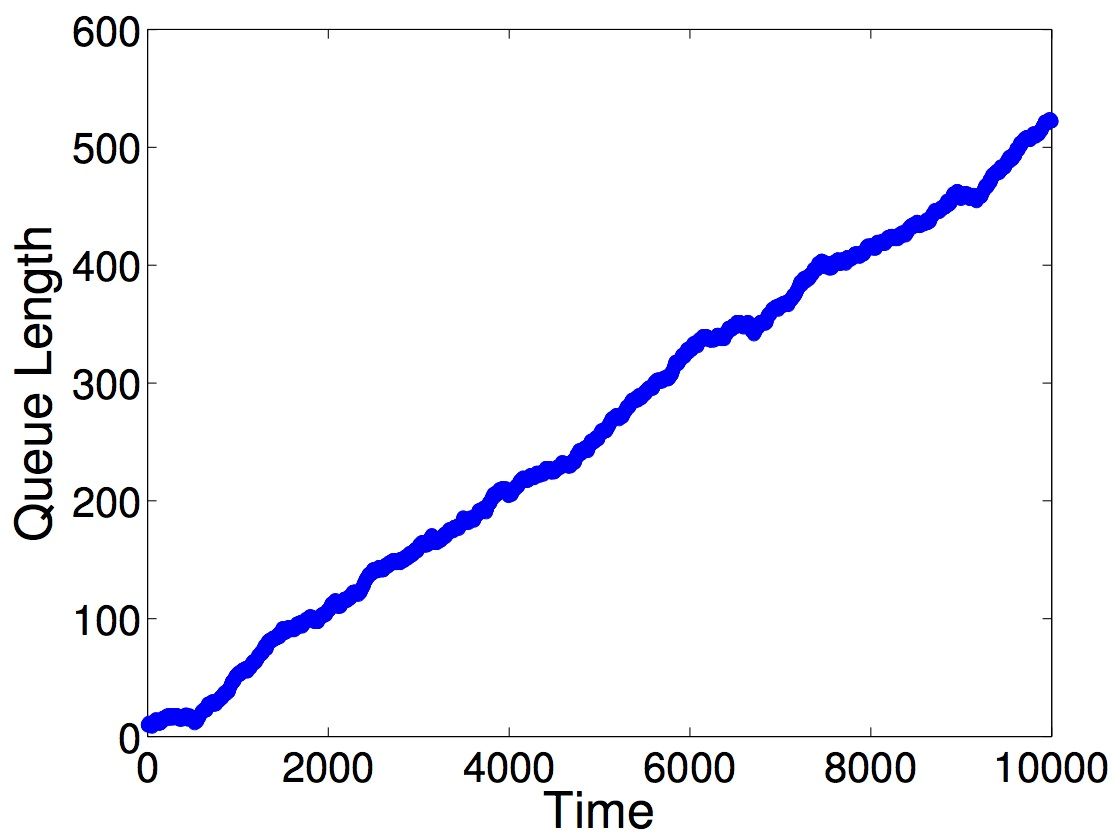
\includegraphics[width = 2.75in]{Figures/Bernoulli_3.jpg} &
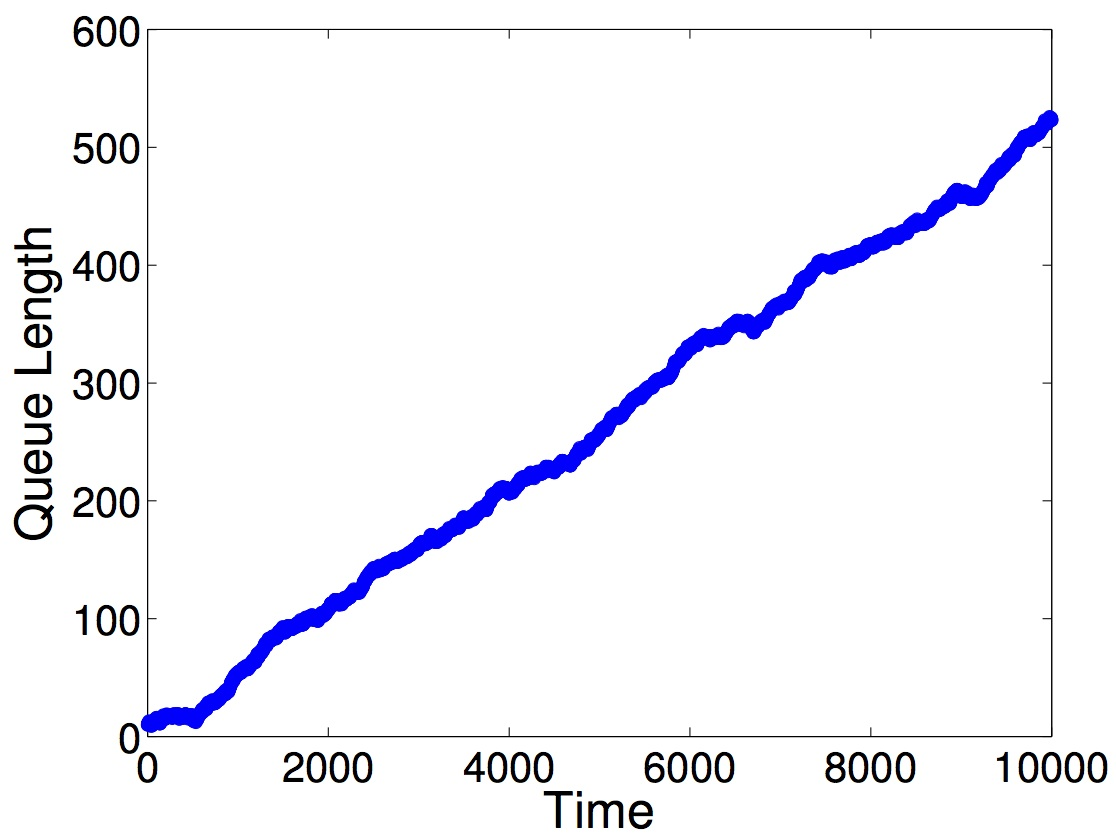
\includegraphics[width = 2.75in]{Figures/Bernoulli_4.jpg} \\
(a) & (b)
\end{array}$
\caption{Queue lengths as a function of time for (a) $Q_1$ and (b) $Q_2$ for the priority max weight allocation with Bernoulli arrival process for the unstable case with $p_1 = 0.6$ and $p_2 = 0.5$.}
\label{fig:BernoulliUnstable}
\end{figure}






We next consider a deterministic arrival process with alternating arrivals. The arrival rates are $\lambda_i = 0.5 $ and the queues are stable. The corresponding queue lengths are shown in Figure \ref{fig:Deterministic}.

\begin{figure}[h]
\centering
$\begin{array}{cc}
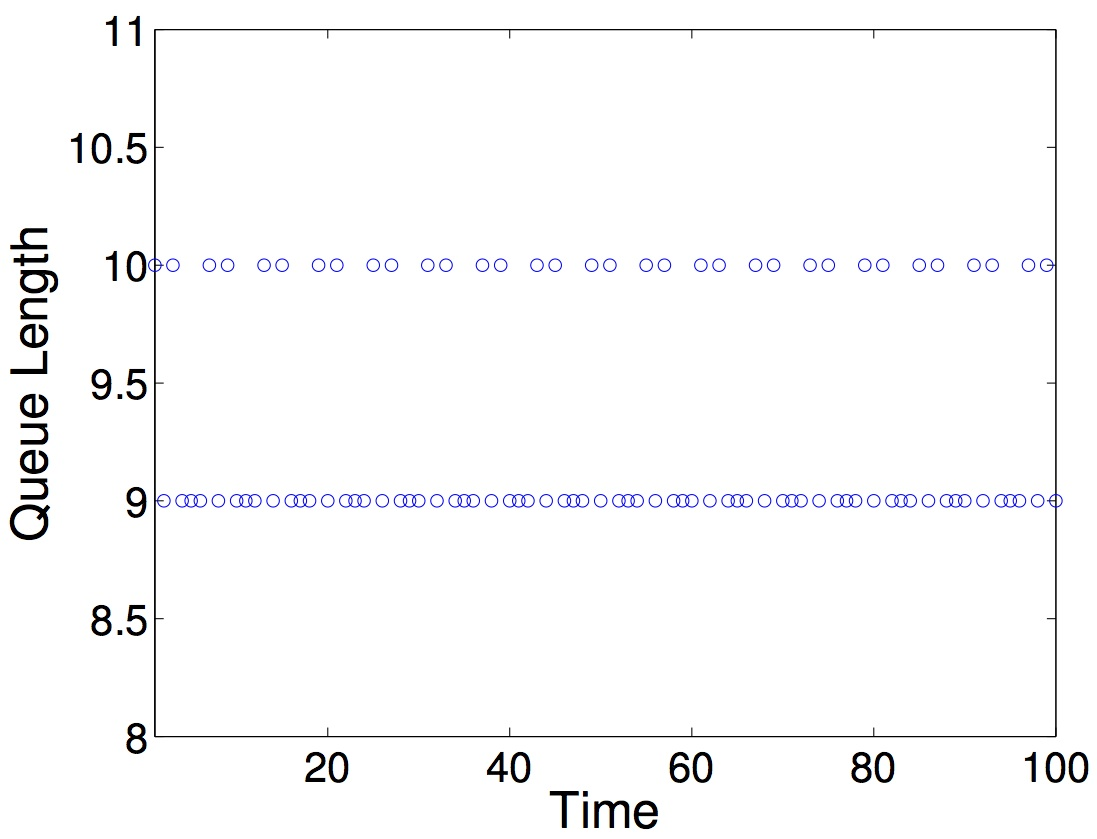
\includegraphics[width = 2.75in]{Figures/Deterministic_1.jpg} &
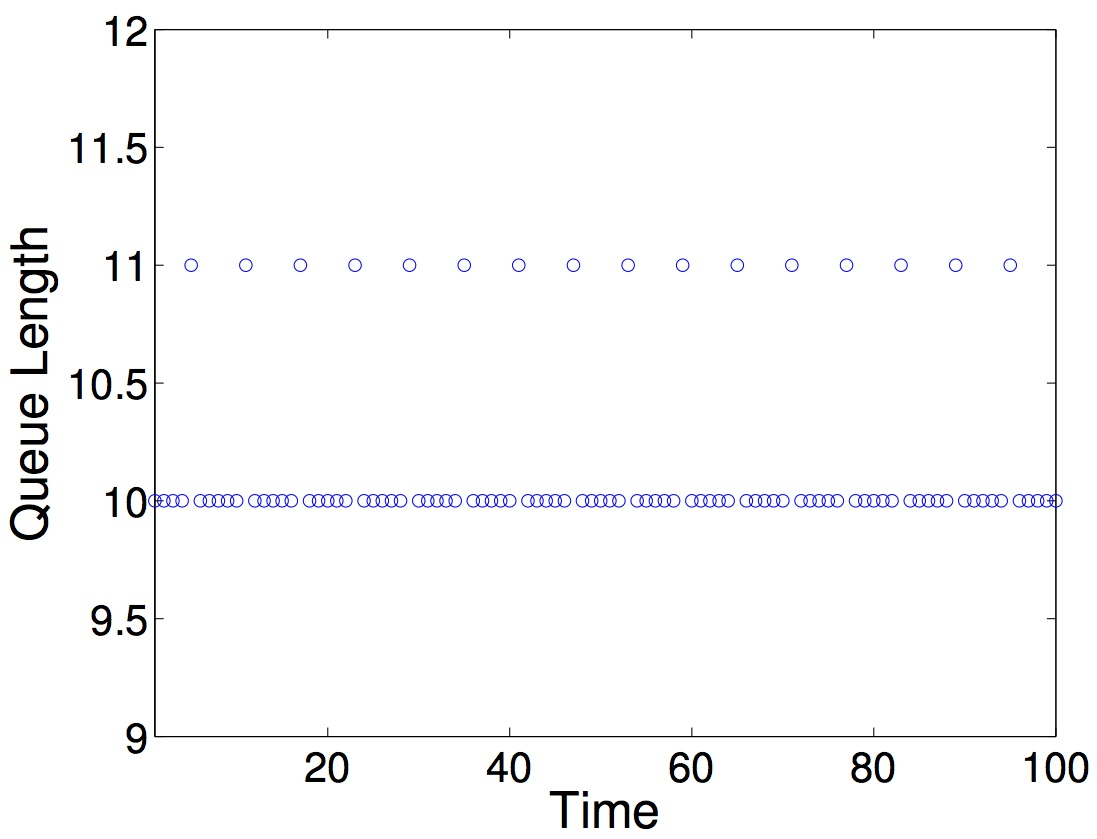
\includegraphics[width = 2.75in]{Figures/Deterministic_2.jpg} \\
(a) & (b)
\end{array}$
\caption{Queue lengths as a function of time for (a) $Q_1$ and (b) $Q_2$ for the priority max weight allocation with the deterministic arrival process with rates being $0.5$ each.}
\label{fig:Deterministic}
\end{figure}







\section{Backlog Queues}
\label{sec:BacklogQueues}
We next consider queues with infinite backlogs for which we model Person A's frustration to increase with the number of consecutive waiting intervals and the length of each such interval, rather than him leaving the system. An associated cost function would be a convex increasing function of slope greater than unity which favours a more interleaved service. For instance, if we can send two bits in four seconds to Person A, the cost pertaining to $\{1,0,1,0\}$ is lesser than that of $\{1,1,0,0\}.$ This follows since 
$kf(1) < f(k)$ for any $k$. 
Among all allocation policies with the same $\mu_1$, the one that interleaves is the best.

\subsection{A Renewal Reward Approach}

If we say that a renewal occurs whenever Person A is served, then the time average cost to the system can be seen as a renewal reward process which, by the renewal reward theorem, equals the ratio of the  expected cost per cycle to the length of the cycle. Since $\mu_1$ is the rate at which Person A is served, we see that the expected length of the cycle is $\frac{1}{\mu_1}$ and the cost per cycle due to Person A is $f\left(\frac{1}{\mu_1}-1\right)$ and cost per cycle due to Person B is $1$. Thus the total cost per cycle is the weighted average sum of these costs given by  
\begin{align}
\label{eqn:BacklogRate}
\frac{\alpha_1f\left(\frac{1}{\mu_1}-1\right)+\alpha_2}{1/\mu_1} ~=~ \alpha_1 \mu_1 f\left(\frac{1}{\mu_1}-1\right)+\alpha_2 \mu_1.
\end{align}
%
%
%
%
%
%\clearpage
%
%
%
%%\section*{Case 3: Backlog queues}
%For backlog queues, since the concept of stability no longer holds, we consider only satisfying Person A with the appropriate rate $\mu_1$. Since on average, Person A is served once in $\frac{1}{\mu_1}$ seconds, and Person B is served once in $\frac{1}{\mu_2}$ seconds, we see that the average cost per cycle incurred will be
%\begin{equation}
%\label{eqn:BacklogCost}
%\alpha_1 \displaystyle\frac{ f\left(\frac{1}{\mu_1}-1\right)}{\frac{1}{\mu_1}} + \alpha_2 \frac{\left(\frac{1}{\mu_2}-1\right)}{\frac{1}{\mu_2}},
%\end{equation}
%where we have considered a linear cost for Person B pertaining to (\ref{eqn:CostB}). Since the channels are perfect and there is infinite backlog, we have $\mu_1 + \mu_2 = 1$, and hence (\ref{eqn:BacklogCost}) can be written in terms of $\mu_1$ alone as follows
%\begin{align}
%\label{eqn:BacklogRate}
%\alpha_1 \mu_1 f\left(\frac{1}{\mu_1}-1\right) + \alpha_2 (1-\mu_1)\left(\frac{1}{1-\mu_1}-1\right),
%\end{align}
%which can be simplified to 
%\begin{align}
%\label{eqn:BacklogRate}
%\alpha_1 \mu_1 f\left(\frac{1}{\mu_1}-1\right) + \alpha_2 \mu_1.
%\end{align}
The optimal $\mu_1 \in [0,1]$ for (\ref{eqn:BacklogRate}) will then decide the allocation rates. Once $\mu_1$ is known, the most interleaved service per cycle is the best allocation policy. 

\subsection{Example: The Squared-Error Loss}

For the squared-error loss function, that is, $f(x) = x^2,$ which is an increasing convex function, and whose slope is greater than 1 for all positive integers, the loss in \eqref{eqn:BacklogRate} is given by 
\begin{align*}
\alpha_1 \mu_1\left(\frac{1}{\mu_1}-1\right)^2 + \alpha_2 \mu_1,
\end{align*}
which simplifies to 
\begin{align*}
\alpha_1 \left(\frac{1}{\mu_1}+\mu_1 -2\right) +\alpha_2 \mu_1.
\end{align*}
Taking the derivative and equating to $0$, we get 
\begin{align*}
\mu_1 = \left(\frac{\alpha_1}{\alpha_1 + \alpha_2}\right)^{1/2},
\end{align*} 
which is the optimal $\mu_1 \in [0,1].$ In the extreme cases when $\alpha_1 = 0$ and $\infty$, we see that $\mu_1 = 0$ and $1$, respectively, as one would intuitively expect.

\section{Conclusions}
In this work, we considered an rate allocation policy that optimally satisfies the needs of 2 different types of users. We modeled the dissatisfaction of the users in 2 ways, and presented allocation policies that minimise the corresponding loss and hence improving quality of experience. We showed that a simple modification of the max-weight algorithm provides a stable and optimal allocation policy, the stability of which was confirmed by the Lyapunov criterion. Further, we showed that the renewal reward theorem can be employed to convert a stochastic optimisation problem to a deterministic one involving only the service rates. 

A future direction could be generalising the number of users of each type, and the number of bits sent per time slot could be changed to a more general range rather than $\{0,1\}$. Another aspect that can be addressed is the fading channel, which can be modeled by a Bernoulli or a Rayleigh fading channel. The cost pertaining to Type 2 user can, in this context, be dependent on a threshold quality (rate) level.


\bibliographystyle{IEEEtran}
\bibliography{Reference}

















%
%\clearpage
%~ \clearpage
%
%\section*{Case 2: General $L$, perfect channel}
%
%
%\subsection*{A cost based approach}
%$\gamma_2(t) = \{ \text{number of bits  $< R$ in } \{b_2(\tau)\}_{\tau=0}^t\}$
%
%
%\section*{Case 3: $L=1$, Channel fading} $C_i = \text{Ber}\{p_i\}$\\
%\noindent $\lambda_1 + \lambda_2 < p_1(1-p_2) + p_2(1-p_1)+p_1p_2.$\\
%
%\noindent When both are active, select $C_1$ with probability $\beta.$
%
%\section*{Case 4: General $L$, Channel fading}
%














\end{document}
